\section{Introduction}\label{sec:intro}

% Need a paragrapgh or two to explain why the tool is interesting and
% significant should be provided.

\dReach{} is a bounded reachability analysis tool for hybrid systems. It encodes
bounded reachability problems of hybrid systems as first-order
formulas over the real numbers, and solves them using
$\delta$-decision procedures in the SMT solver \dReal{}~\cite{}. \dReach{} is
able to handle a wide range of highly nonlinear hybrid systems. It has
scaled well on various realistic nonlinear models from biomedical and
robotics applications~\cite{}. Figure~\ref{fig:prostate-example} highlights 
some of its features: 
on the left is an example of some nonlinear dynamics that \dReach{} can handle, 
and on the right a visualized counterexample generated by \dReach{} on this model.
\begin{figure}[!h]
  \subfloat[An example of nonlinear hybrid system model: off-treatment
  mode of the prostate cancer treatement model~\cite{}\label{subfig-1:prostate}]{
    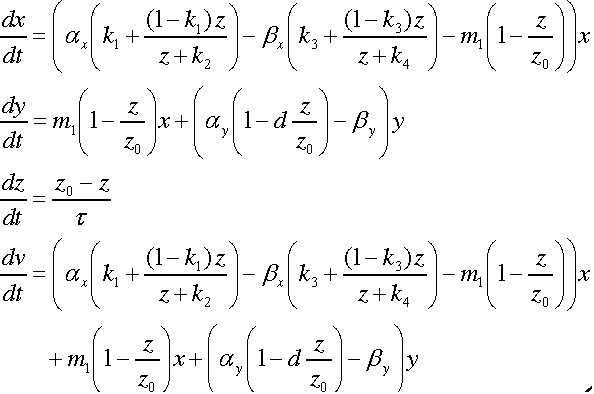
\includegraphics[width=0.48\textwidth]{images/prostatebw-mode2.pdf}
  }
  \hfill
  \subfloat[Visualization of a generated counterexample. Change in the shade of colors represents discrete mode changes.]{%
    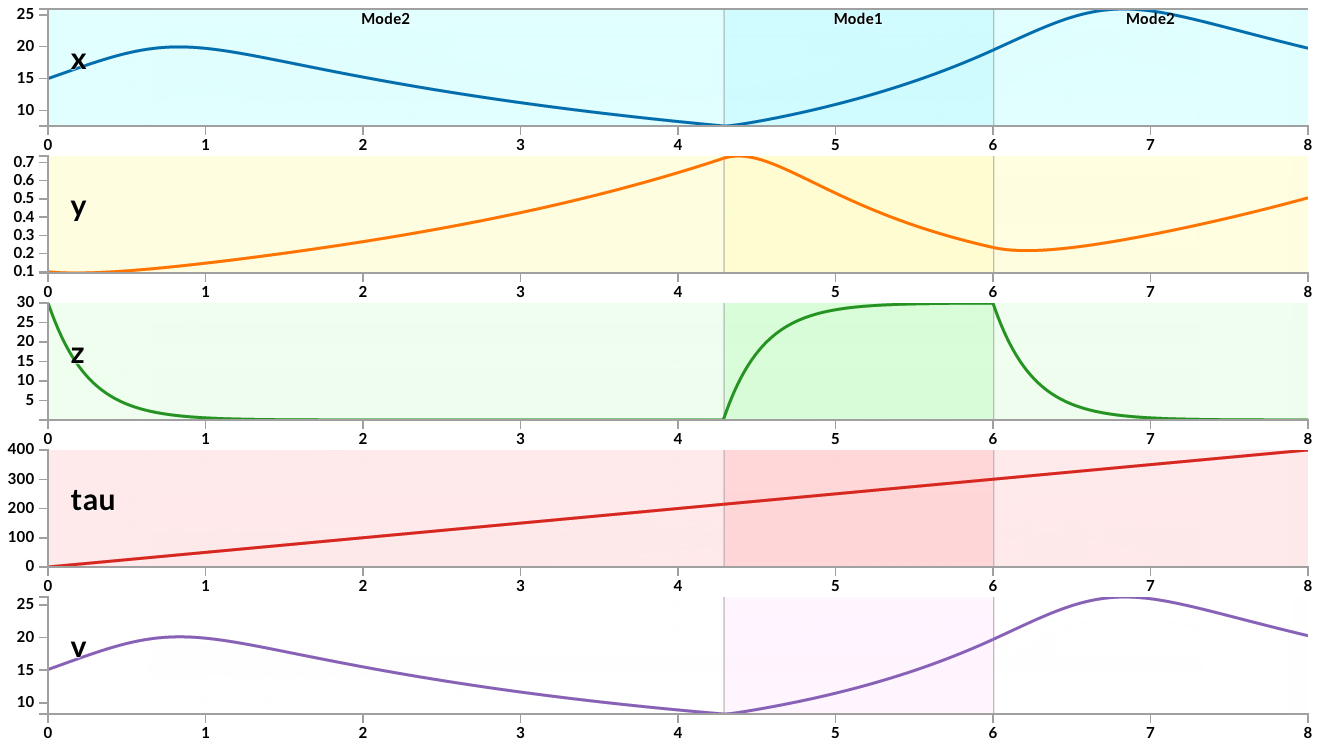
\includegraphics[width=0.48\textwidth]{images/prostate}
  }
  \caption{An example of nonlinear dynamics and counterexample-generation.}
  \label{fig:prostate-example}
\end{figure}

It is well-known that the standard bounded reachability problems for
simple hybrid systems are already highly
undecidable~\cite{DBLP:conf/rex/AlurD91,DBLP:conf/hybrid/AlurCHH92}. To bypass this difficulty, we defined the framework
of $\delta$-complete analysis of reachability for general nonlinear hybrid systems~\cite{}. 
We have shown that bounded $\delta$-reachability is in fact decidable for a wide range of hybrid systems, with reasonable
complexity bounds~\cite{}. We give a brief review of some basic definitions in
Section~\ref{sec:delta-reachability}.

Several key features of \dReach{} separate it from other existing tools in this domain~\cite{DBLP:journals/jlp/FranzleTE10,
DBLP:conf/icons/HerdeEFT08,DBLP:conf/cav/GulwaniT08,DBLP:conf/rtss/ChenAS12}. For instance:  
%insert explanations for each item.
\begin{itemize}
\item Any nonlinear dynamics. Any logic formulas in the signature for describing jumps, conditions, etc.
\item Faithful encoding of invariants as $\exists\forall$ problems.
\item No explicit storage of reachable states but perform property guided search for concrete trajectories.
It avoids the state explosion in representing the full reachable set. This is analogous to the difference between SAT-based
model checking and symbolic model checking.
\item It provides a general framework that can make full use of exisiting reachable set computation algorithms and logic solving.
\end{itemize}
%Realistic hybrid systems involves nonlinear ODEs with transcendental
%functions. \dReach{} allows users to specify a hybrid system in a
%nonlinear signature as it is without linearizing or overapproximating
%it. Users can provide the tool with a numerical error bound $\delta$,
%a bounded time horizon $[0, T]$, and a maximum number of mode switches
%$k$ for the analysis. As a result of analysis, \dReach{} will return
%either \textbf{$\delta$-sat} with a concrete counterexample, or
%\textbf{unsat} which does not involve numerical errors. We also
%provide a visualization for the $\delta$-sat case to help
%understand the analysis result.

% TODO: Need to diiferentiate this paper from FMCAD paper
%  - FMCAD: underlying solving techniques for SMT with ODEs
%  - TACAS: tool, encoding, using solver...

The paper is structured as follows.

\newpage
%%% Local Variables:
%%% mode: latex
%%% TeX-master: "main"
%%% End:
